\documentclass[10pt]{beamer}
\usepackage{uglixbeamer}
\title{Listes chaînées}
\subtitle{Chapitre 16}
\author{NSI2}


\begin{document}

\maketitle

\begin{frame}{Caractéristiques}
	\begin{itemize}
		\item \alert{Rien à voir avec le type \mintinline{python}{list} de Python...}
		\item Structure linéaire : éléments rangés « les uns à la suite des autres ».
		\item Cet ordre est un ordre \alert{sur les places} des éléments, pas sur les éléments.
	\end{itemize}
\end{frame}
\begin{frame}{Type \mintinline{python}{list} de Python}
    \begin{center}
        \includegraphics[width=8cm]{img/Liste}
    \end{center}
    Pour simplifier, une variable de type \mintinline{python}{list} est un peu comme un \alert{tableau} : Les adresses des éléments sont connues et l'accès à tel ou tel élément se fait en une seule fois (on dit « en temps constant»).
\end{frame}
\begin{frame}{Liste}
    \begin{center}
    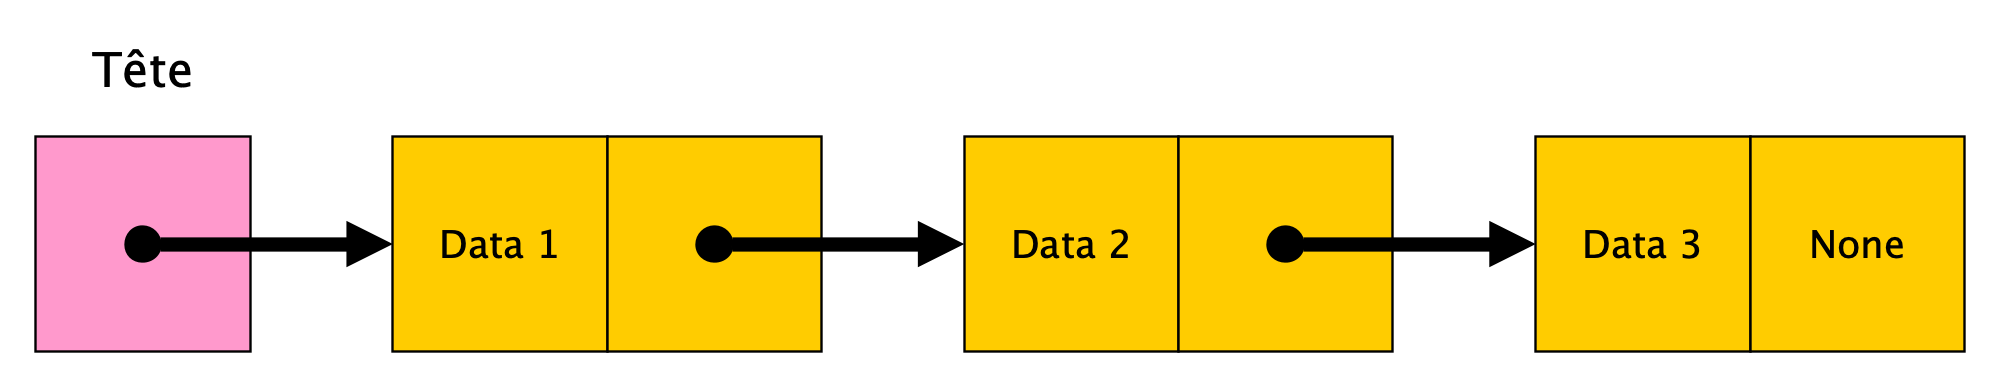
\includegraphics[width=8cm]{img/liste_chainee1}
\end{center}
La structure de donnée \textit{liste} est bien différente.
\end{frame}

\begin{frame}{Interface}
	Interface de la structure de donnée
	\begin{itemize}
		\item \textit{liste\_vide()}\\ renvoie une... liste vide.
		\item \textit{element(liste, position)}\\ renvoie l'élément à la position donnée.
		\item \textit{longueur(liste)}\\renvoie la longueur de la liste.
		\item \textit{supprimer(liste, position)}\\ supprime l'élément de la liste qui est à la position donnée.
		\item \textit{inserer(liste, valeur, position)}\\ insère la valeur à la position donnée.
	\end{itemize}
	On convient que, comme en Python, la première position est 0.
\end{frame}
\begin{frame}{Pré-conditions}
	Ce sont les conditions qui doivent être vérifiées pour pouvoir se servir de l'interface. Par exemple :\\

	\textit{element(liste, position)} n'est défini que si $position<longueur(liste)$.\\

	Il y en a d'autres, elles sont faciles à trouver.
\end{frame}
\begin{frame}{Axiomes (hors programme)}
	En théorie on doit énoncer des propriétés appelées \textit{axiomes}, pour que la structure de donnée soit cohérente. Par exemple :
	\begin{itemize}
		\item \textit{longueur(liste\_vide)=0};
		\item si liste est non vide et que $0\leqslant k \leqslant longueur(liste)$ alors $$longueur(supprimer(liste, k))=longueur(liste)-1$$
		\item si  $0\leqslant k \leqslant longueur(liste)$ alors $$longueur(inserer(liste, valeur,k))=longueur(liste)+1$$
	\end{itemize}
	Il y en a d'autres, nous n'en parlerons pas
\end{frame}
\begin{frame}{Intérêt des pré-conditions et des axiomes}
	\begin{itemize}
		\item Connaître les pré-conditions est utile lors de l'implémentation, pour \alert{lever des erreurs}.
		\item Les axiomes peuvent servir à fabriquer des tests unitaires.
	\end{itemize}
\end{frame}

\begin{frame}{Implémentations}
	\begin{itemize}
    	\item	Avec une variable de type \mintinline{python}{list}. (Trop facile !)
    	\item	De même, encapsulé dans un objet
        \item 	En POO.
    \end{itemize}
\end{frame}

\begin{frame}[fragile]{Liste chaînée}
	Pour disposer d'une liste chaînée non vide, il faut un lien vers le premier élément de la liste : la tête.\\
	Chaque élément de la liste doit contenir :
	\begin{itemize}
		\item une valeur (on supposera qu'elles sont toutes du même type);
		\item un lien vers la cellule suivante, le dernier élément ne contenant pas de lien (on notera \mintinline{python}{None} l'absence de lien).
	\end{itemize}
	\begin{center}
	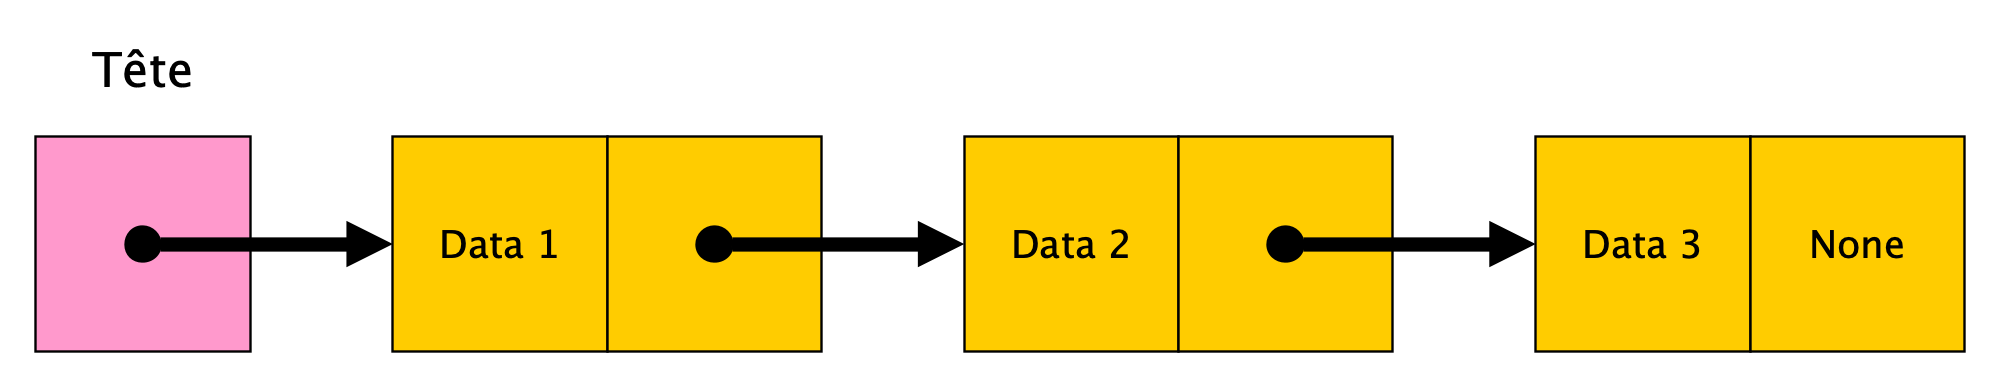
\includegraphics[width=8cm]{img/liste_chainee1}
	\end{center}
\end{frame}
\begin{frame}{Fonction liste\_vide}
	\begin{center}
		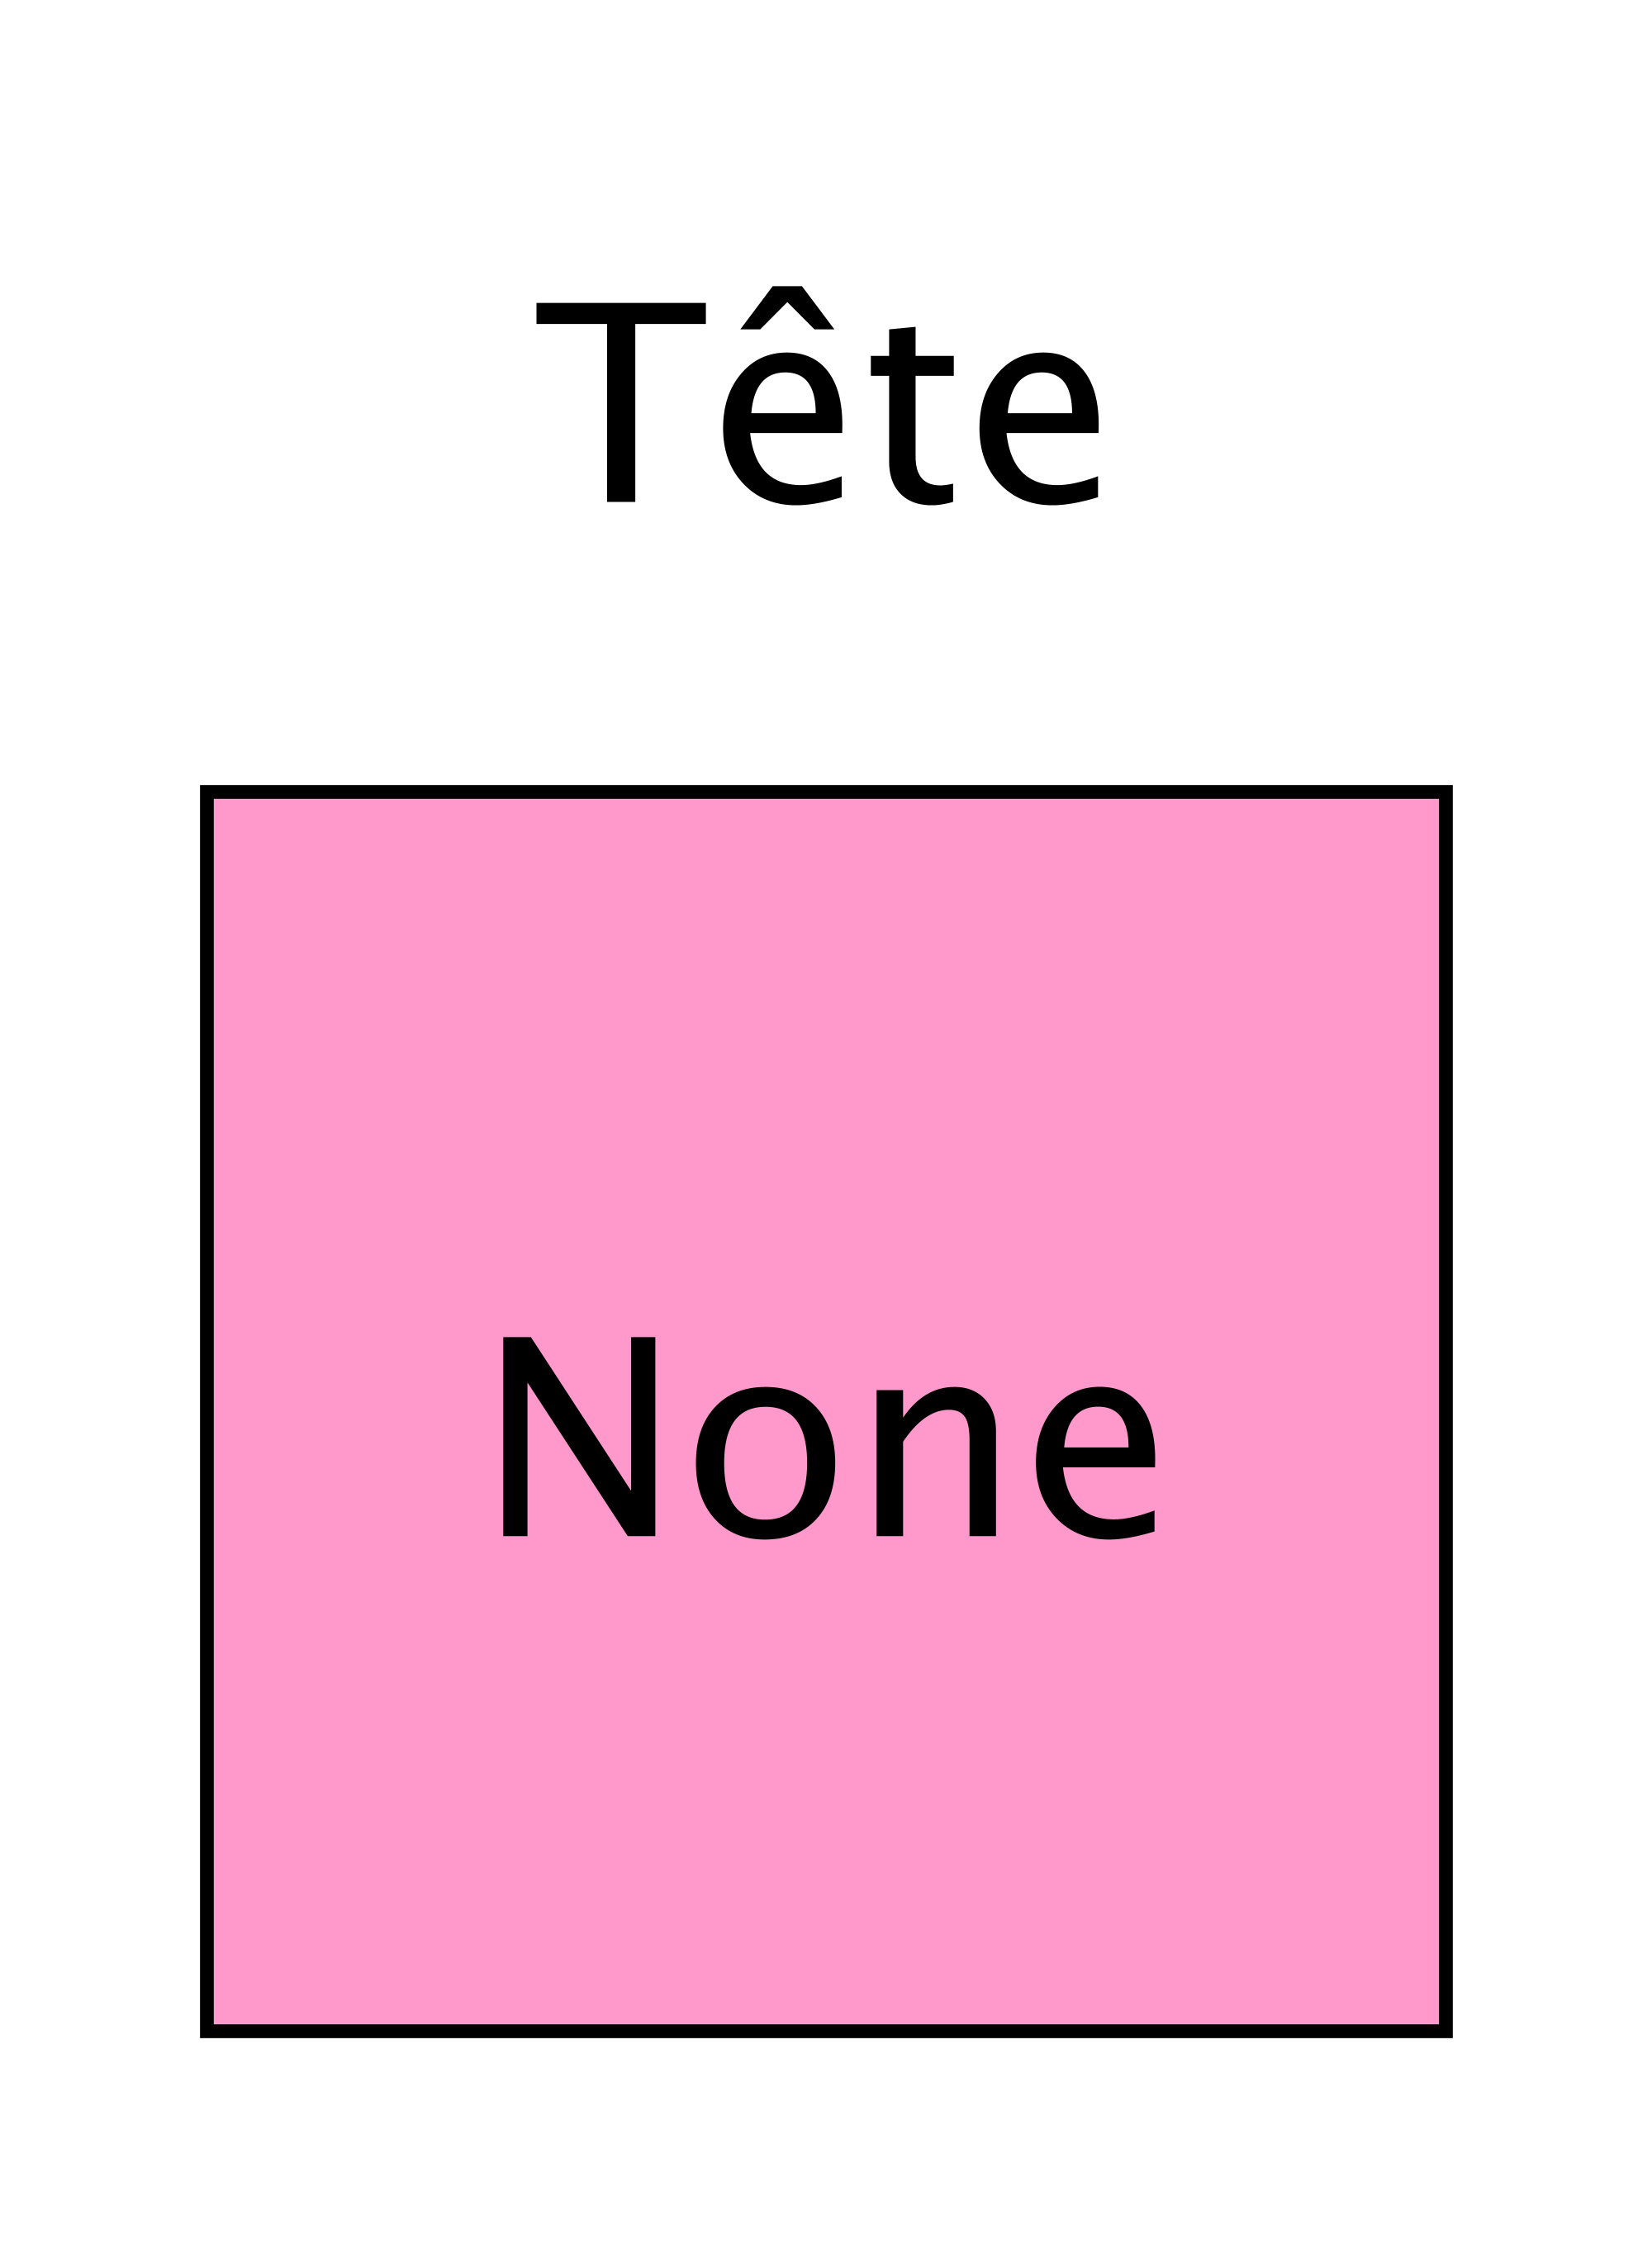
\includegraphics[width=2cm]{img/liste_vide}
	\end{center}
\end{frame}
\begin{frame}{Fonction element}
	\textit{element(liste,position)} parcourt la liste en commençant par la tête et passant au maillon suivant tant que nécessaire.
\end{frame}
\begin{frame}{Fonction longueur}
	\textit{longueur(liste)} parcourt la liste en commençant par la tête jusqu'au dernier maillon (qui n'a pas de successeur) et en comptant combien il y en a.
\end{frame}

\begin{frame}[fragile]{Supprimer}

\only<1>{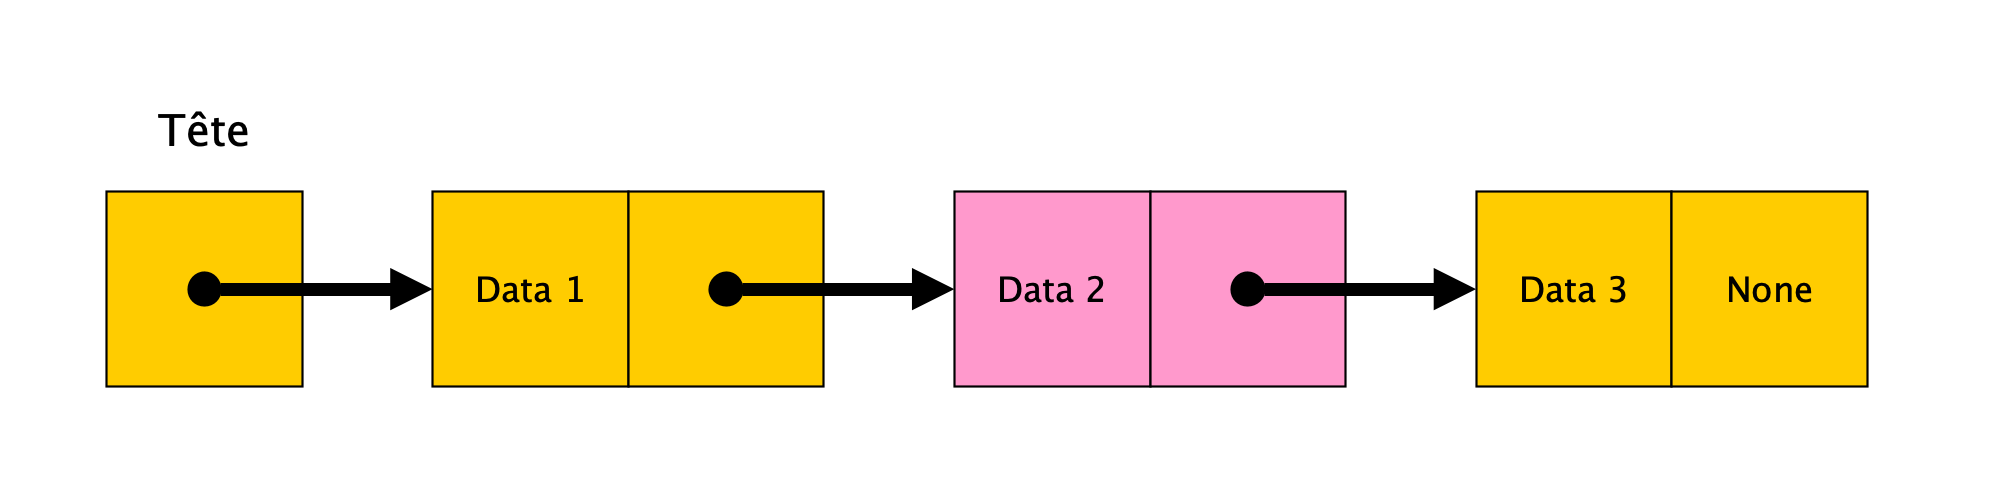
\includegraphics[width=10cm]{img/suppr1_0}\\ On veut supprimer un élément.}
\only<2>{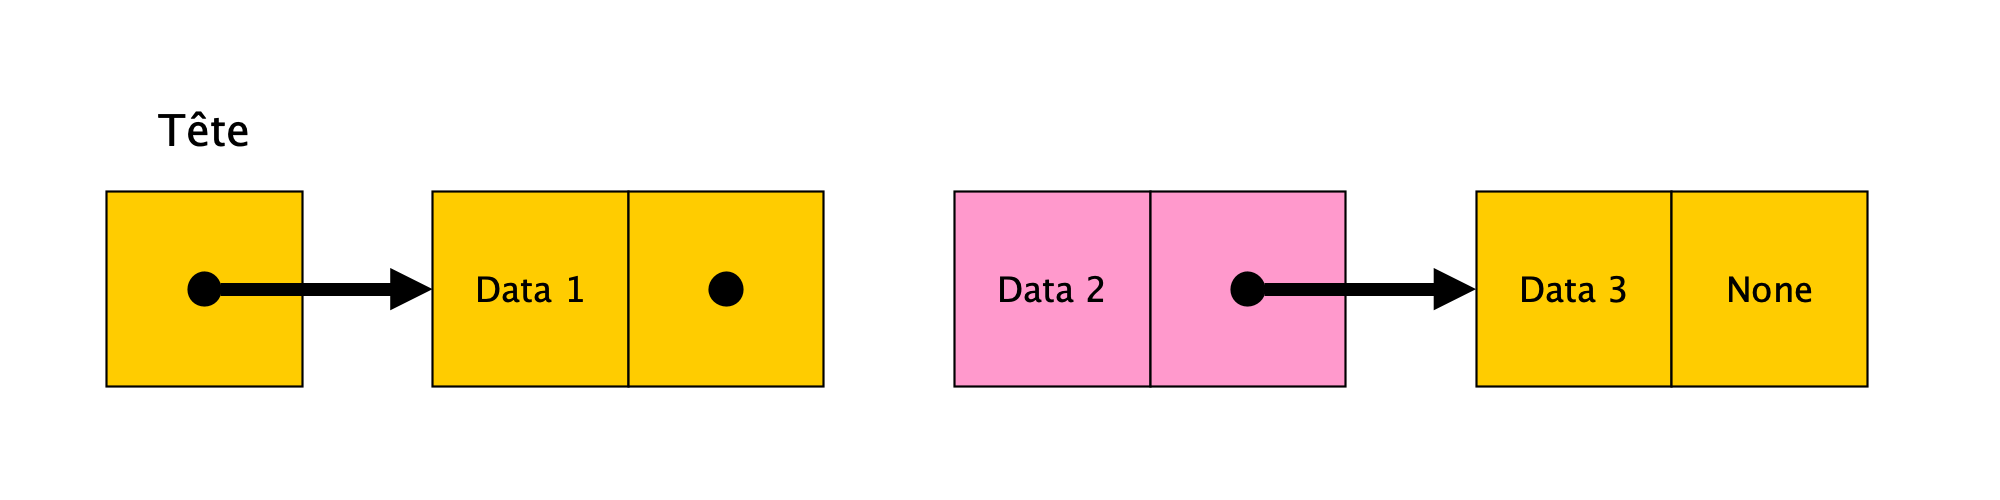
\includegraphics[width=10cm]{img/suppr1_1}\\ On le déconnecte de son prédécesseur (ou de la tête).}
\only<3>{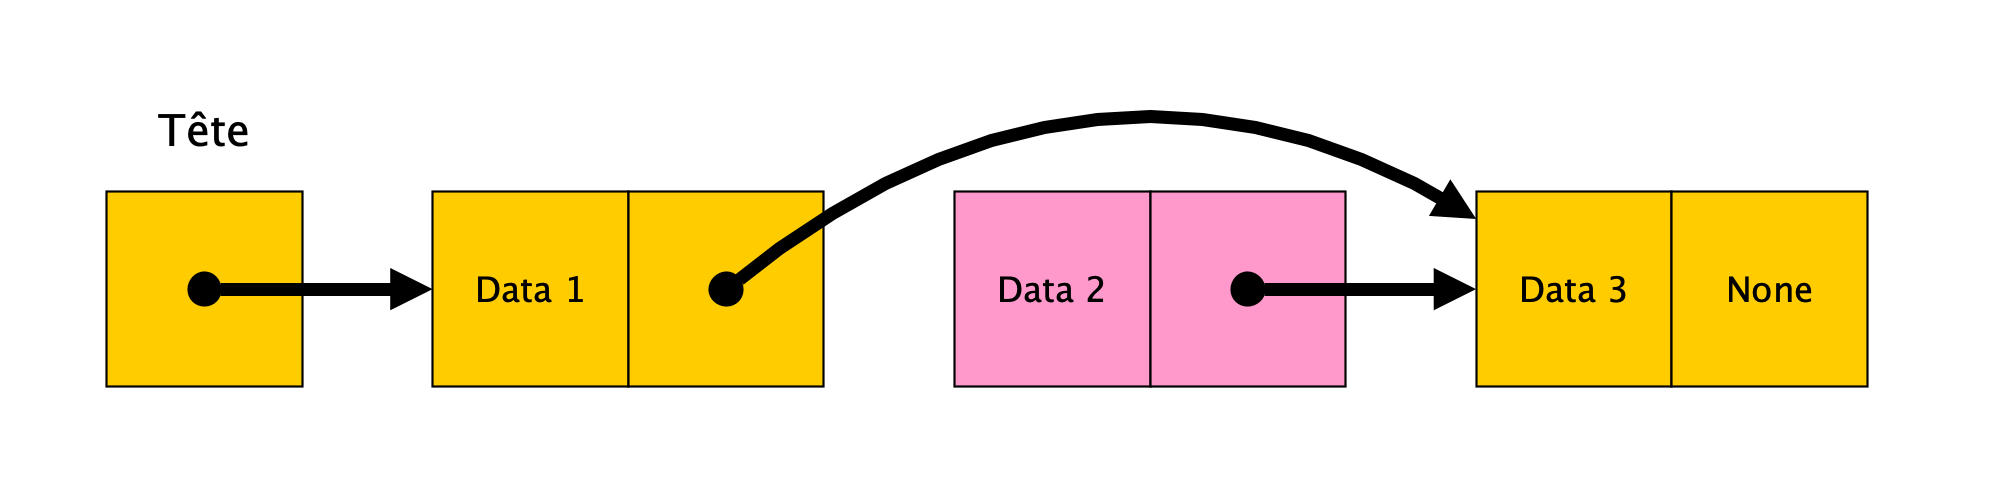
\includegraphics[width=10cm]{img/suppr1_2}\\ On connecte son prédécesseur  à son successeur (s'il y en a un).}
\only<4>{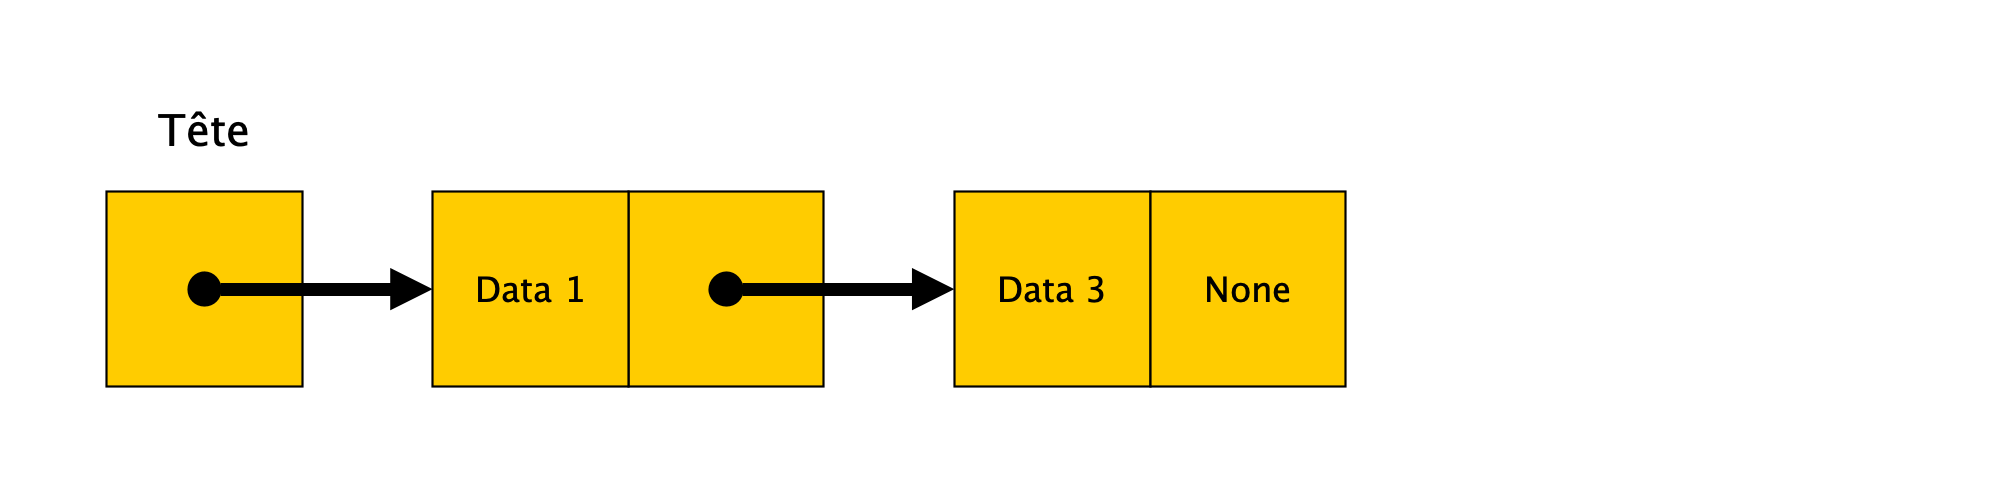
\includegraphics[width=10cm]{img/suppr1_3}\\ On « efface » définitivement l'élément (avec un \mintinline{python}{del} par exemple).}
\end{frame}

\begin{frame}[fragile]{Inserer}

	\only<1>{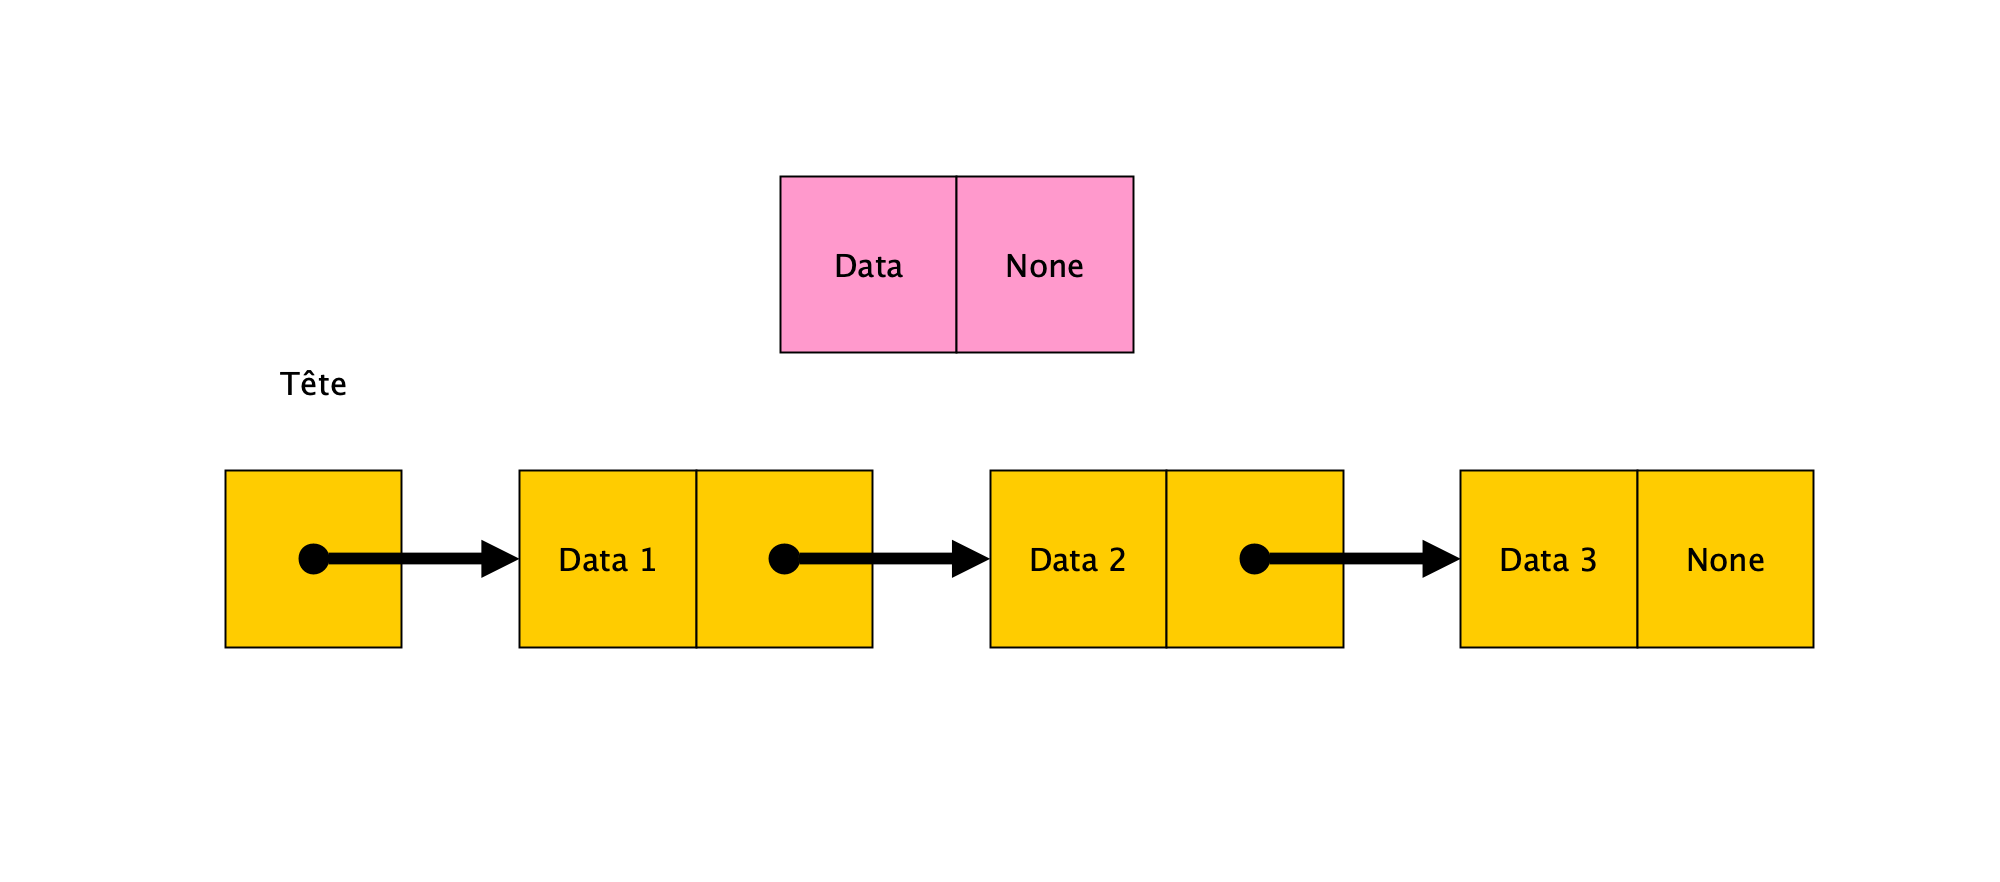
\includegraphics[width=10cm]{img/insert0}\\ On veut insérer un élément.}
	\only<2>{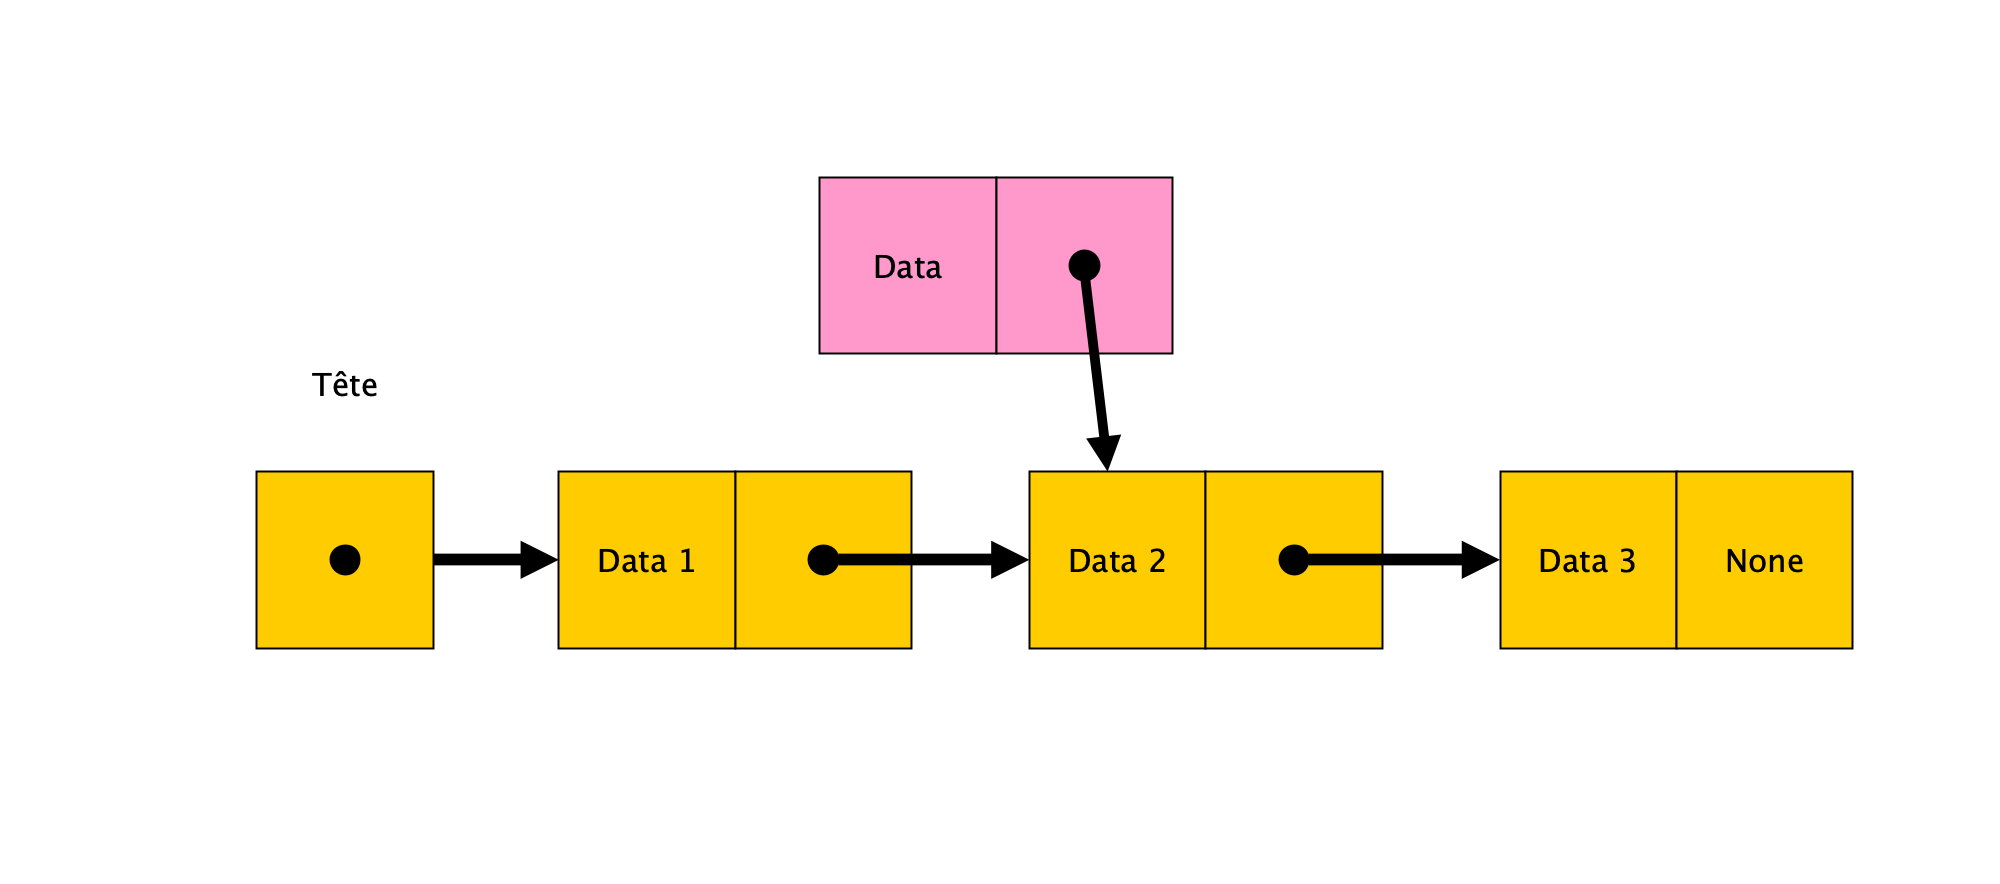
\includegraphics[width=10cm]{img/insert1}\\ On le connecte à son (éventuel) futur successeur.}
	\only<3>{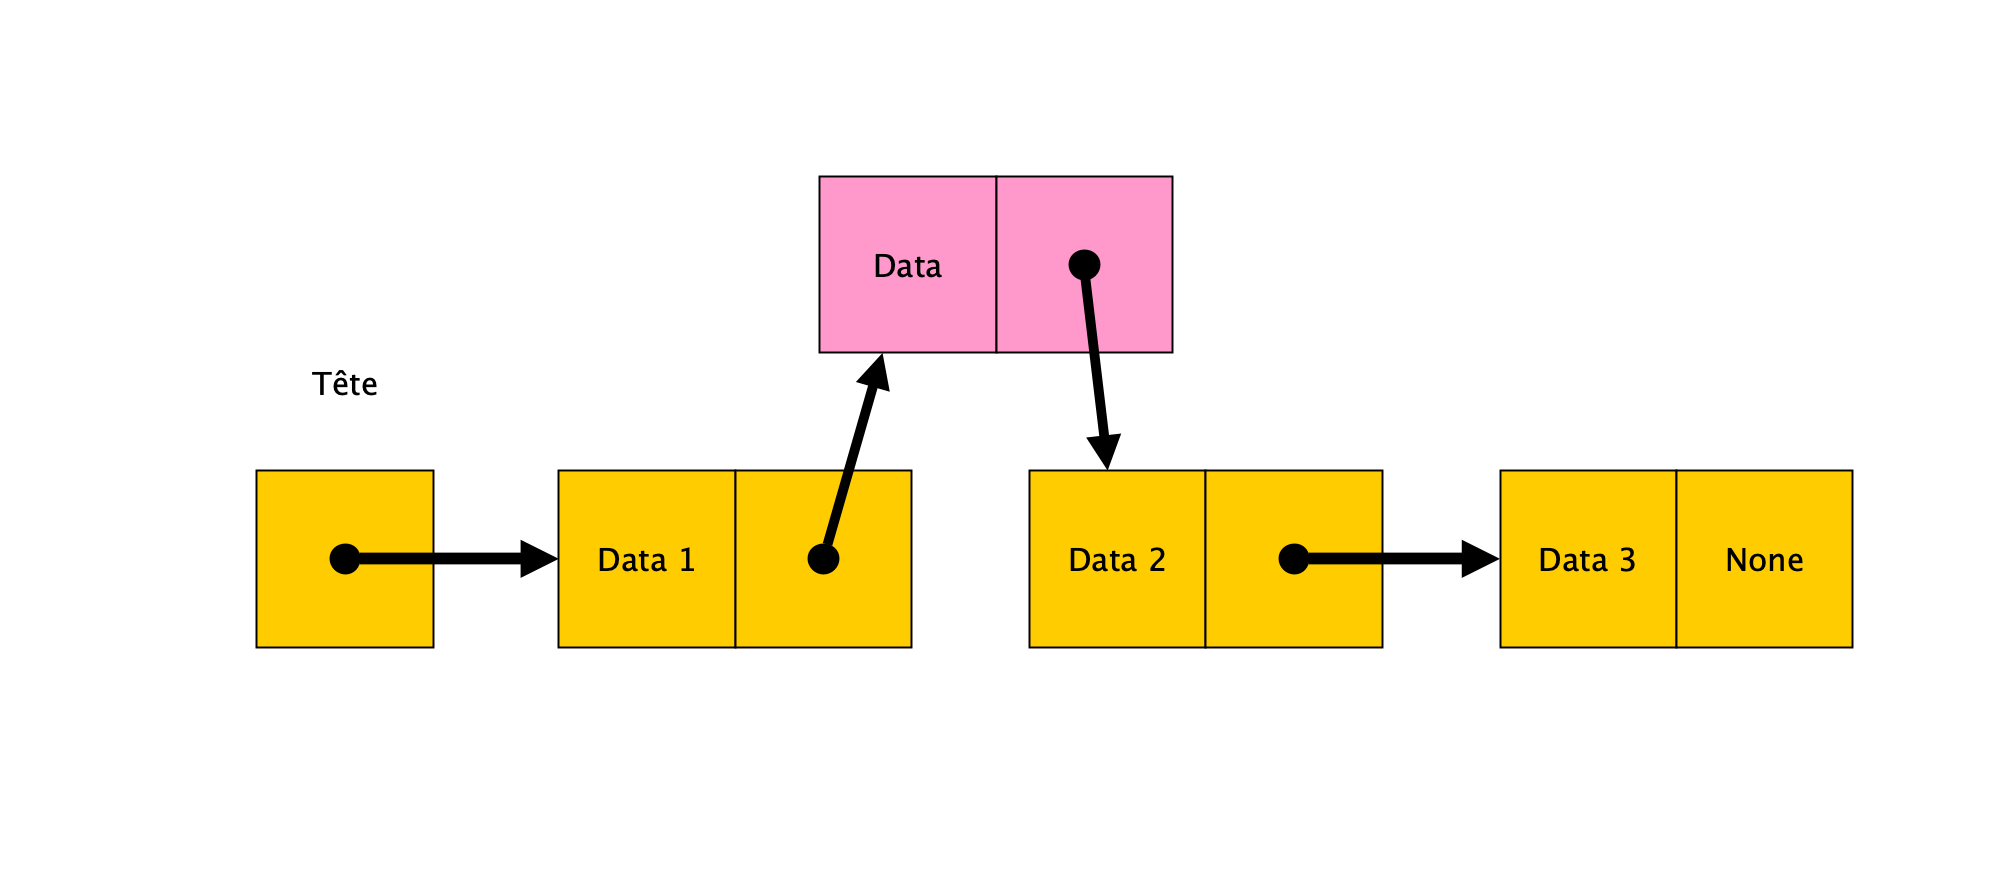
\includegraphics[width=10cm]{img/insert2}\\ On le connecte à son futur prédécesseur (ou tête).}
	\only<4>{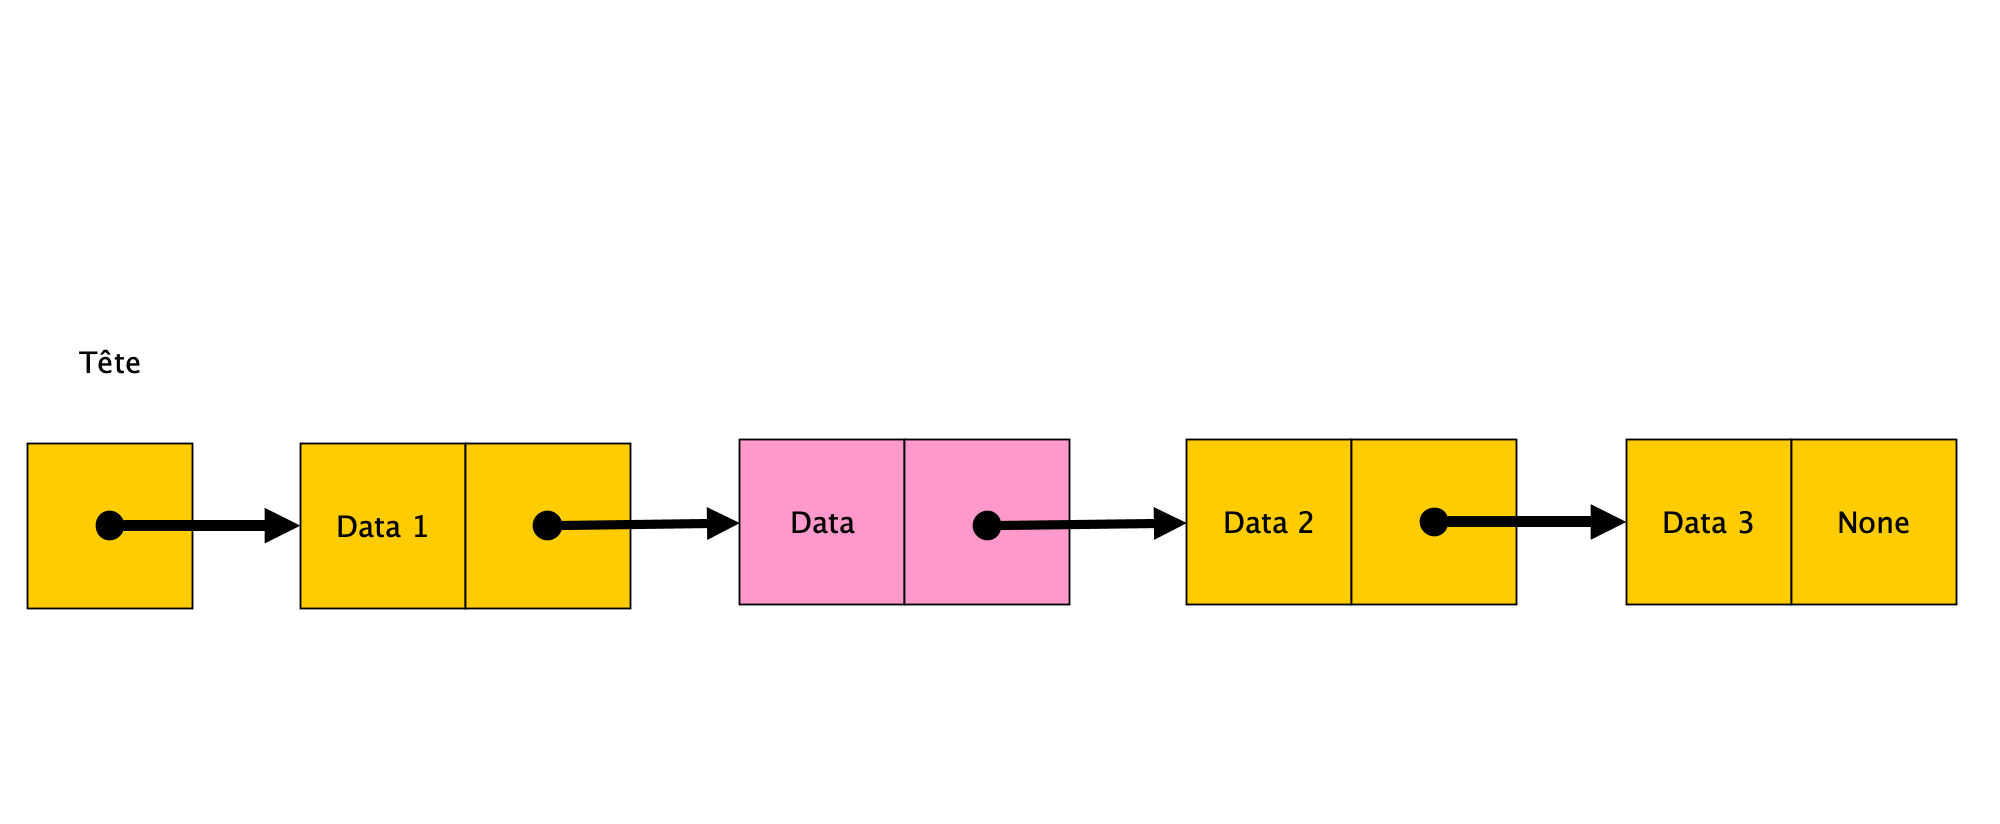
\includegraphics[width=11cm]{img/insert3}\\ Et voilà !}
\end{frame}

\begin{frame}[fragile]{Quelques différences \mintinline{python}{list} / liste chaînée}
\begin{itemize}
    \item \textbf{temps de suppression du premier élément :}  \begin{itemize}
        \item Très court pour une liste chaînée
        \item Proportionnel à la taille de la liste Python
    \end{itemize}
    \item \textbf{temps de suppression du dernier élément :}  c'est le contraire
    \item \textbf{temps d'accès à la longueur :} immédiat pour la liste Python et proportionnel à la longueur de la liste chaînée
    \item \textbf{temps d'accès à un élément :} immédiat pour la liste Python et proportionnel à la place de l'élément pour la liste.
\end{itemize}
\end{frame}
\end{document}